El proyecto de investigación ARTEMIS es una iniciativa interdisciplinaria que reúne el trabajo de varios estudiantes de diferentes especialidades y campos. Este enfoque colaborativo permite abordar el proyecto desde diversas perspectivas, enriqueciendo así el desarrollo y la implementación de soluciones innovadoras. ARTEMIS se centra en el diseño y desarrollo de aplicaciones digitales interactivas. Estas han sido específicamente desarrolladas para realizar terapias de estimulación emocional a través del arte y la música, utilizando la tecnología como vehículo principal. Además, estas aplicaciones están diseñadas para ser intuitivas y accesibles, permitiendo a los usuarios interactuar con ellas de manera sencilla. Este proyecto tiene como objetivo integrar las últimas innovaciones tecnológicas con prácticas terapéuticas tradicionales, para potenciar los beneficios emocionales y psicológicos de los pacientes. A pesar de que cada uno de los estudiantes que conforman el equipo se ha centrado en líneas de investigación particulares, todos comparten objetivos comunes que han guiado sus esfuerzos hacia una meta colectiva.

Para contribuir al conocimiento científico y hacer funcionales las terapias diseñadas, las aplicaciones permiten la configuración por edades y patologías. Se definen pruebas psicométricas\footnote{Los test psicométricos son largos ya que consisten en alrededor de 30-40 preguntas. Al final de cada aplicación o sesión, se realizan preguntas rápidas del tipo termómetro.} al inicio y al final de la actividad, y los datos recogidos\footnote{La definición del perfil del paciente implica una entrevista entre el terapeuta y el paciente, donde se indaga acerca de su historia musical, gustos y características relacionadas con la música. El terapeuta será el encargado de introducir una serie de datos en la aplicación para optimizar esta fase.} de los pacientes se almacenan para su posterior consulta por el terapeuta. Los datos recogidos incluyen la edad, el nivel escolar, si se ha estudiado algún instrumento y el instrumento preferido del paciente. El perfil del paciente determina la complejidad musical en, por ejemplo, la composición interactiva. Un perfil con menos experiencia musical tendrá la capacidad de entender una complejidad musical menor o menos disonante, mientras que un perfil con más experiencia puede manejar una armonía más elaborada. Es importante mencionar que estas aplicaciones tienen una función de doble usuario en la que tanto el terapeuta como el paciente participan simultáneamente, cada uno con un rol específico. El terapeuta actúa como instructor, guiando al paciente en su interacción con la aplicación. 

La primera fase del proyecto ARTEMIS se ha enfocado en el tratamiento de la ansiedad infantil, utilizando la tecnología como vehículo para la transición emocional, complementándose con terapias tradicionales basadas en musicoterapia. La estructura de las sesiones terapéuticas es modular y se puede adaptar a las necesidades individuales del paciente. Cada sesión comienza con la definición del perfil del paciente y luego se selecciona una o más actividades vinculadas directamente a las líneas de investigación previamente definidas, en las que profundizaremos más en detalle en los próximos párrafos. Dentro de cada actividad, se han desarrollado una o más aplicaciones con distintos enfoques, que pueden ser utilizadas en función de las observaciones del terapeuta. Las actividades que han servido como punto de partida para el desarrollo de estas aplicaciones, y que han dado lugar a las líneas de investigación, son:

\begin{itemize}
	\item \textbf{Actividad 1 - Psicoeducación emocional:} esta primera actividad se enfoca en entender la emoción, específicamente la ansiedad, y en cómo combatirla. El educador, que en este caso es el terapeuta, proporciona de manera concisa información científica relevante para responder a preguntas importantes. El paciente recibe una serie de herramientas que le ayudan a identificar, comprender y manejar la ansiedad.
	\item \textbf{Actividad 2 - Relajación guiada mediante la respiración:} el terapeuta, con la ayuda del soporte digital, guía al paciente a realizar ejercicios de relajación centrados en la respiración. El paciente sincroniza sus respiraciones con la interacción tecnológica, aportando un elemento artístico que acompaña la respiración.
	\item \textbf{Actividad 3 - Ordenar pensamientos a través del ritmo:} el paciente se centra en utilizar el ritmo como herramienta para organizar sus pensamientos y emociones. Bajo la guía del terapeuta, se establece un escenario rítmico que permite al paciente explorar y organizar sus ideas y sentimientos de una manera ordenada, respetando siempre su subjetividad.
	\item \textbf{Actividad 4 - Improvisación:} se basa en la completa libertad del paciente, donde, a través de la improvisación musical, el paciente debe expresar su estado de ánimo.
	\item \textbf{Actividad 5 - Repetición de patrones rítmicos:} el paciente debe escuchar y repetir patrones rítmicos con la mayor precisión posible con el objetivo de controlar la impulsividad. 
\end{itemize}

Estas actividades constituyen la base sobre la que se han construido para las distintas aplicaciones, respaldadas por las líneas de investigación. Estas líneas se han establecido para abordar los objetivos del proyecto desde una perspectiva multidisciplinaria, uniendo las cuatro áreas de estudio: arte, tecnología, música y terapias de estimulación emocional. Las líneas de investigación son las siguientes:

\begin{itemize}
	\item Musicoterapia y narrativa audiovisual.
	\item Musicoterapia y arte digital.
	\item Musicoterapia y composición interactiva.
	\item Musicoterapia y diseño de videojuegos (serious games).
	\item UX/UI interacción y branding.
\end{itemize}

Abordaremos cada línea de investigación individualmente, indagando en profundidad en sus aplicaciones derivadas. Específicamente, la aplicación más relevante para este Trabajo de Fin de Grado se encuentra en la línea de investigación de diseño de videojuegos con musicoterapia. Dejaremos esta para el final con el fin de explicarla en mayor detalle, ya que es él núcleo principal de este trabajo.

\section{Musicoterapia y narrativa audiovisual}

La narrativa audiovisual es una parte integral del proyecto de investigación. Está presente en todas las aplicaciones, en mayor o menor medida, y actúa como un vínculo entre todas ellas. El objetivo de contar una historia es proporcionar información al paciente de manera que pueda sentirse identificado y conectar directamente con sus emociones. Dado que estamos estudiando la ansiedad, es importante explicar al paciente cómo funciona e involucrarlo en la explicación integrada en forma de historia. Hemos definido tres elementos en la narrativa que están directamente relacionados con este enfoque, y cuyo objetivo es involucrar activamente al paciente.

\begin{itemize}
	\item \textbf{Personaje principal:} es el elemento más crítico de la narrativa. Su función es actuar como un espejo que permite al paciente identificarse, y sirve como guía para el mismo. Este personaje es una especie de Pepito Grillo\footnote{Pepito Grillo es un personaje de ficción creado para Las Aventuras de Pinocho (\cite{LADP:1883}), que Walt Disney Pictures, actual Walt Disney Studios, adaptó en 1940 en la película de animación Pinocho. En la cultura popular, Pepito Grillo representa una figura de confianza a quien recurrimos para obtener consejo. Esta figura nos ayuda a identificar nuestros errores y no teme cuestionarnos cuando nos equivocamos.}, cuyo objetivo es ayudar al paciente a comprender su problema y a encontrar una solución.
	\item \textbf{Nivel de explicación:} dependiendo de la edad a la que se dirige la narrativa, el nivel de profundidad debe variar y adaptarse\footnote{Por ejemplo, los niños pequeños suelen utilizar el pensamiento mágico, como un duende malo que nos pone nerviosos, mientras que los adolescentes necesitan ejemplos más concretos y realistas.}. El objetivo es lograr que el paciente se identifique con el ejemplo situacional que la historia propone. Para que esto suceda, es esencial usar analogías para explicar las leyes del mundo.
	\item \textbf{Píldoras mínimas:} para que la historia sirva como un nexo cohesivo entre las aplicaciones, debe quedar claro cuál es el objetivo de la actividad específica que se va a realizar. Debe responder a la pregunta: ¿Cuál es la finalidad de lo que estoy a punto de hacer?
\end{itemize}

Todos estos elementos se centran en lo que se conoce como inmersión contextual. Esto implica el estudio del contexto de los pacientes para introducir elementos que se ajusten a las circunstancias de cada uno. El objetivo es promover una identificación adecuada entre el paciente, su situación y la historia.

La historia principal debe unir todas las actividades de forma natural sin perder el objetivo que acabamos de comentar. Esta historia, escrita por Isabel Xiaowei de San Sebastián para ARTEMIS, se puede resumir de la siguiente manera:

\begin{adjustwidth}{100pt}{0pt}
	\noindent "\textit{El protagonista es un ser del bosque que nació de una flor, gracias al poder de una ninfa. La diosa Artemis ha perdido su magia y el protagonista ayuda a recuperarla. Su misión es buscar semillas de diente de león perdidas en el bosque para entregárselas a la ninfa, quien las transforma en flores. En su travesía, se encuentra con varios desafíos, representados por actividades terapéuticas, que debe completar para avanzar. El nivel no concluye hasta que se completan todas las actividades. Una vez finalizado un nivel, el protagonista puede repetirlo o continuar con la historia. Las ninfas, en intervalos regulares, se reúnen con las distintas flores de cada emoción que han creado a partir de las semillas y se las entregan a Artemis. Cada emoción se representa como una planta distinta, personalizando así la estética del personaje con diferentes plantas. Existe una escala del dolor que, dependiendo del nivel de ansiedad del paciente, muestra diferentes elementos que ayuden al terapeuta a comprender la situación del paciente.}"
\end{adjustwidth}

La ambientación de esta historia está fuertemente vinculada con la naturaleza, que se asocia con la relajación y vitalidad. Así, los elementos estéticos deben ser coherentes con este tema. Considerando que ARTEMIS se centra en la ansiedad infantil, los elementos estéticos se diseñan para adecuarse a este contexto. Esta estética, repleta de colores vivos y personajes con rasgos de la animación tradicional, busca establecer una conexión con su público objetivo. Como no podemos determinar el género del paciente que utilizará la aplicación, decidimos desde el principio que el personaje debía ser andrógino. En la \autoref{fig:MainCharacterConcept}, observamos que se intentó alcanzar este objetivo desde las primeras propuestas estéticas. La versión final del personaje mantiene la androginia, combinando rasgos humanos con elementos naturales. Se puede comparar la versión inicial con la final en la \autoref{fig:MainCharacter}.

\begin{center}
	\textbf{Fuente:} Realizado por Sergio Calvo, miembro ARTEMIS.
	\vspace{-18pt}
\end{center}

\begin{figure}[h!]
	\centering
	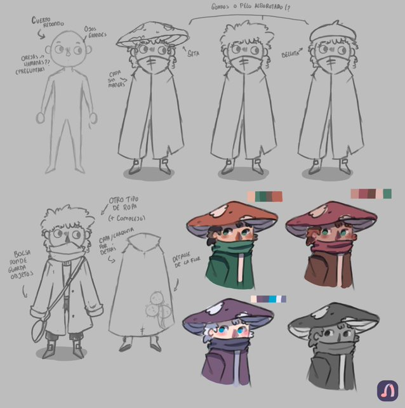
\includegraphics[width=0.4\linewidth]{Figuras/Desarrollo/PersonajesNuevosConcept}
	\caption{Propuesta inicial de personaje principal.}
	\label{fig:MainCharacterConcept}
\end{figure}

\begin{center}
	\textbf{Fuente:} Realizado por Isabel Xiaowei de San Sebastián, miembro ARTEMIS.
	\vspace{-18pt}
\end{center}

\begin{figure}[h!]
	\centering
	\subfigure[Primera iteración del personaje.]{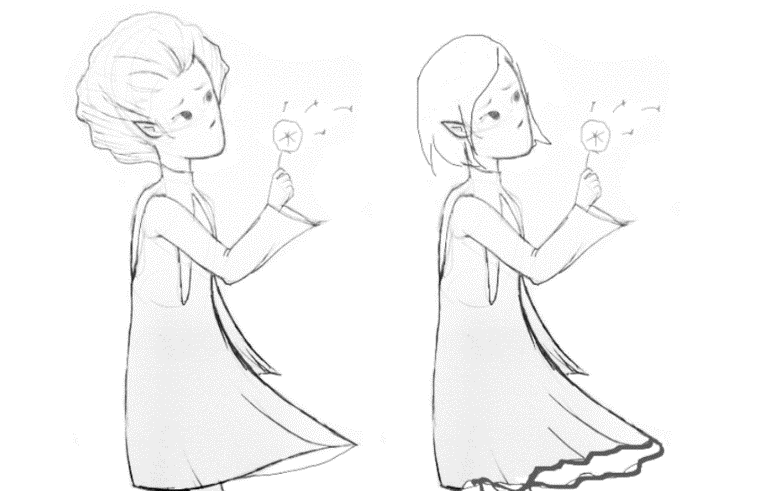
\includegraphics[width=0.4\textwidth]{./Figuras/Desarrollo/PersonajesAntiguos.png}\label{fig:MainCharacterOld}}
	\hfil
	\subfigure[Última iteración del personaje.]{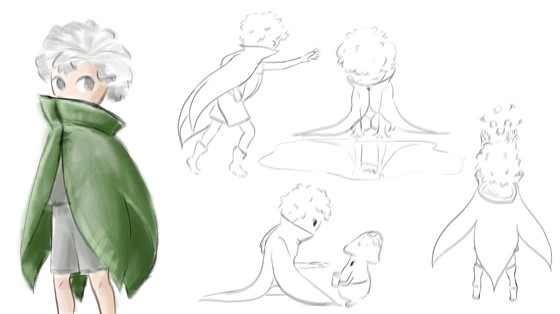
\includegraphics[width=0.4\textwidth]{./Figuras/Desarrollo/PersonajesNuevos.jpg}\label{fig:MainCharacterNew}}
	\caption{Evolución de la conceptualización del personaje principal.}
	\label{fig:MainCharacter}
\end{figure}

Las ninfas, musas y gracias tienen una fuerte relación con la música y pueden ser los personajes identificados con instrumentos que el protagonista encuentra en su aventura. Por esta razón, los personajes secundarios que el protagonista encuentra a lo largo de la narrativa portan instrumentos (como se puede observar en la \ref{fig:InstrumentCharacters}), representando físicamente a estos seres.

\begin{center}
	\textbf{Fuente:} Realizado por Isabel Xiaowei de San Sebastián, miembro ARTEMIS.
	\vspace{-18pt}
\end{center}

\begin{figure}[h!]
	\centering
	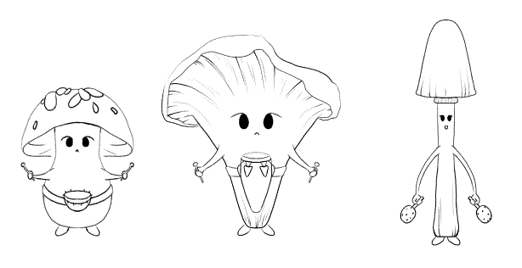
\includegraphics[width=0.3\linewidth]{Figuras/Desarrollo/InstrumentCharacters}
	\caption{Propuesta de concepto de personajes con instrumentos.}
	\label{fig:InstrumentCharacters}
\end{figure}

Antes de concluir esta línea de investigación, es relevante describir el formato que fundamenta esta historia y cómo se lleva a cabo la interacción del paciente bajo la guía del terapeuta. La historia se visualiza a través de un libro ilustrado interactivo. De este modo, el terapeuta puede controlar el ritmo de la historia y, si es necesario, retroceder. Para avanzar, se debe pulsar manualmente el botón de pasar página, permitiendo al terapeuta determinar cuánto tiempo se necesita en cada página, en caso de tener que explicar algún detalle.
La ansiedad tiende a inquietar a quien la padece. Por ello, un sistema que permite adaptar el ritmo de la narrativa a cada situación, permite al terapeuta elegir el enfoque más beneficioso para el paciente en cuestión.

\begin{center}
	\textbf{Fuente:} \citeauthor{LORIRI:2018} (\citeyear{LORIRI:2018}).
	\vspace{-18pt}
\end{center}

\begin{figure}[h!]
	\centering
	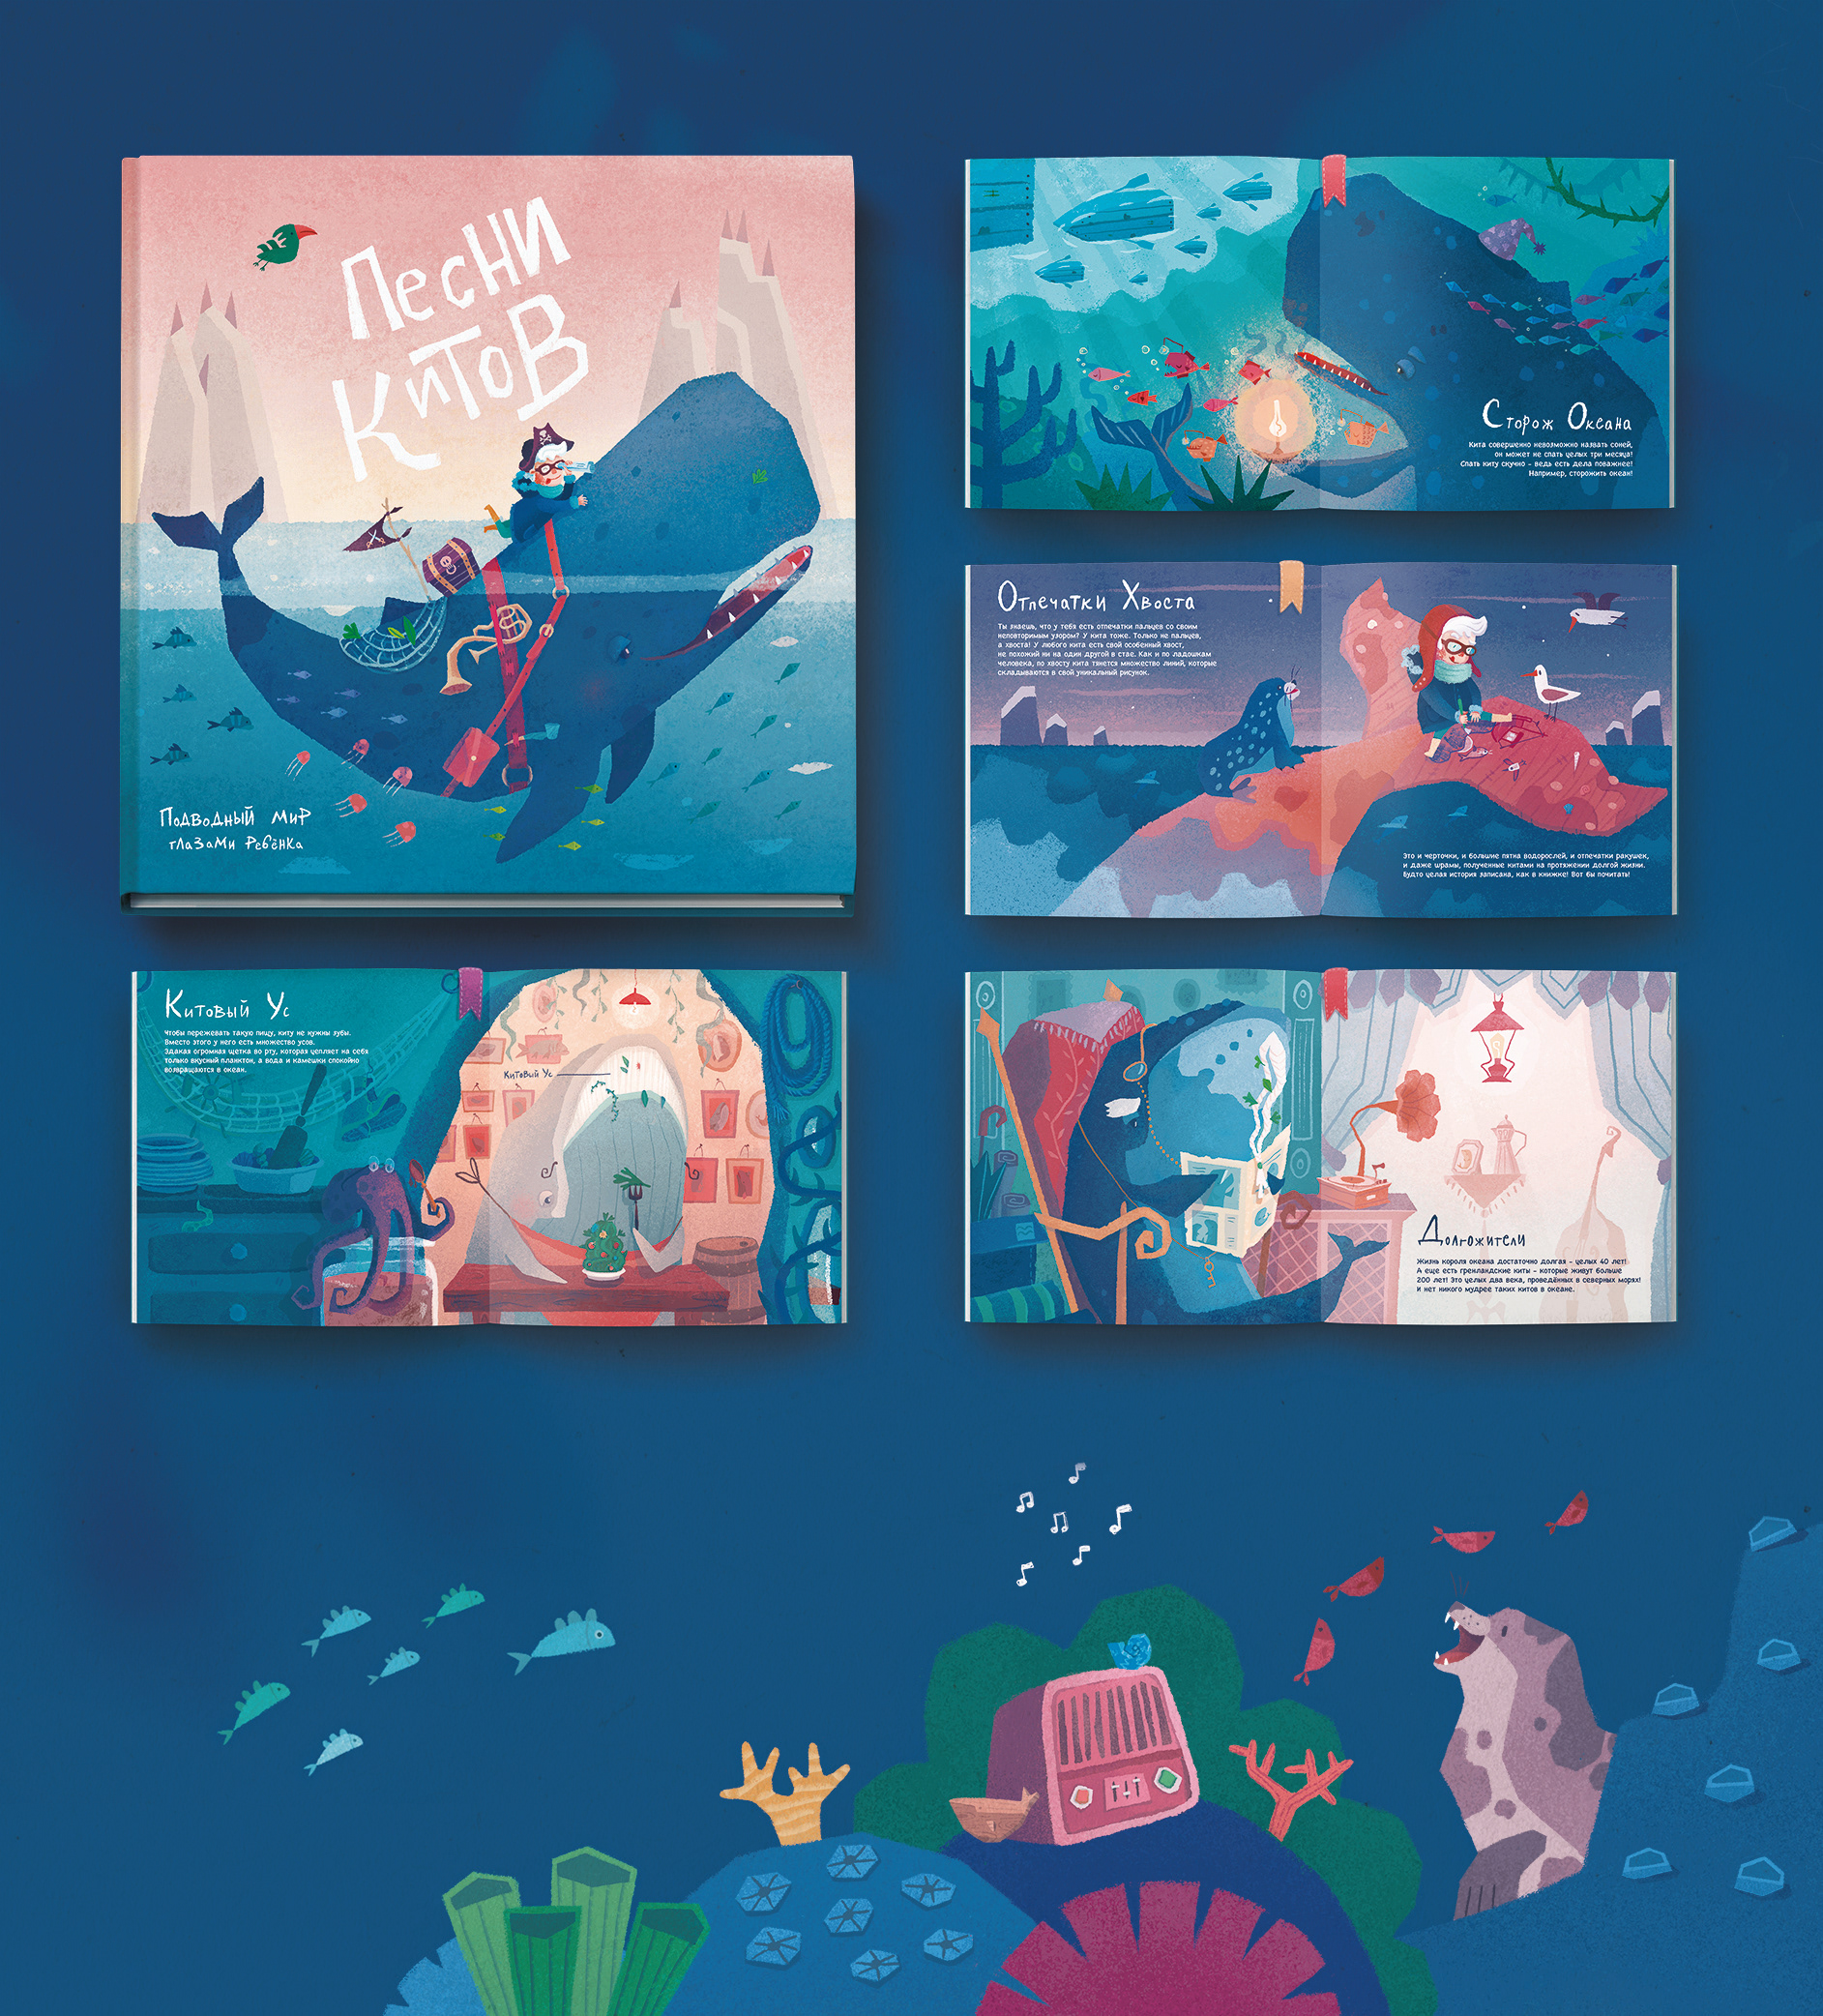
\includegraphics[width=0.4\linewidth]{Figuras/Desarrollo/ImagenReferenciaLibro.jpg}
	\caption{Imagen de referencia de libro interactivo.}
	\label{fig:LoriRiBook}
\end{figure}

\begin{center}
	\textbf{Fuente:} Realizado por Isabel Xiaowei de San Sebastián, miembro ARTEMIS.
	\vspace{-18pt}
\end{center}

\begin{figure}[h!]
	\centering
	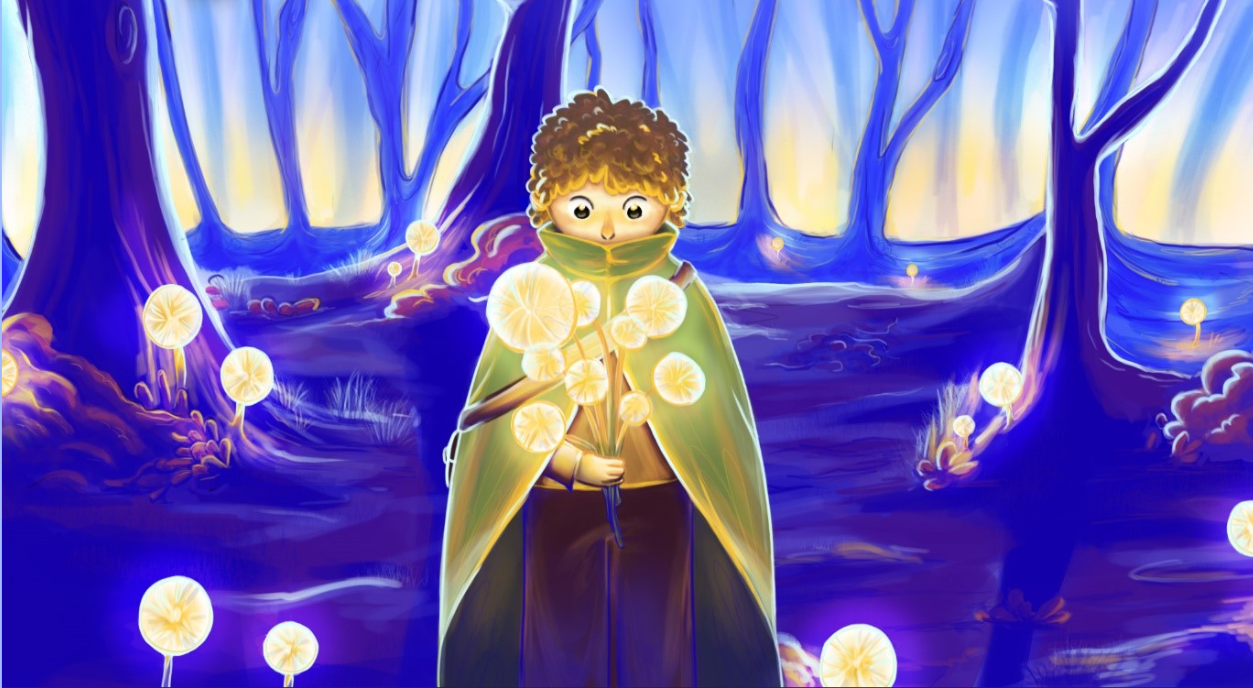
\includegraphics[width=0.5\linewidth]{Figuras/Desarrollo/IlustracionLibro.png}
	\caption{Ilustración de ejemplo del libro ilustrado interactivo.}
	\label{fig:BookIllustration}
\end{figure}

La narrativa es un elemento fundamental para la identificación del paciente con la aplicación. Esta aumenta la eficacia de la terapia en función del grado de inmersión que la tecnología pueda proporcionar en las sesiones de musicoterapia.

\section{Musicoterapia y arte digital}

La línea de investigación en arte digital propone una pieza de arte digital interactiva. Esta pieza, mediante experiencias visuales y música, puede ayudar en la gestión emocional y facilitar la transición de una emoción a otra a través de la interacción del usuario. Los datos de interacción se pueden recoger a través de la información proporcionada por periféricos comunes como una tableta y sus sensores (cámara o pantalla táctil). El objetivo de este recurso es ayudar al paciente a concentrarse y relajarse, enseñándole cómo respirar visualmente en situaciones de ansiedad. La interacción con esta herramienta se realiza mediante pulsaciones táctiles, ya sean cortas o prolongadas, o movimientos de la mano frente a la cámara. Se espera que estas acciones sean guiadas por el terapeuta para alcanzar su objetivo. De esta manera, al no usar un micrófono que puede generar varios problemas dependiendo del tipo de paciente que recibe la terapia\footnote{Usar un micrófono como sistema principal de entrada puede causar problemas en ciertos casos aislados. Las voces más graves producen ondas de sonido que son más difíciles de capturar, por lo que no sería correcto limitar las terapias a personas con voces más reconocibles.}, se evitan complicaciones. En términos de salida de la experiencia, la parte visual se mostrará en la pantalla y la parte musical se emitirá a través de altavoces o auriculares. Las propuestas de visualización para esta pieza se pueden dividir en dos categorías: visual y musical.

\begin{itemize}
	\item \textbf{Apartado visual:} se genera un mar de partículas que oculta un paisaje, siguiendo la línea estética del proyecto. Este paisaje se revela mediante la animación de las partículas, las cuales se ven afectadas por el contacto del dedo del paciente al deslizarse por la pantalla. Este movimiento depende de la longitud de la exhalación.
	\item \textbf{Apartado musical:} se reproduce una melodía relajante de fondo con sonidos que nos recuerdan a la naturaleza (el viento, la vegetación, los animales, etc). Por otro lado, al interactuar con la pieza, también se emite un sonido más fuerte de brisa, que emula la exhalación.
\end{itemize}

\begin{center}
	\textbf{Fuente:} \citeauthor{VAMOSS:2023} (\citeyear{VAMOSS:2023}).
	\vspace{-18pt}
\end{center}

\begin{figure}[h!]
	\centering
	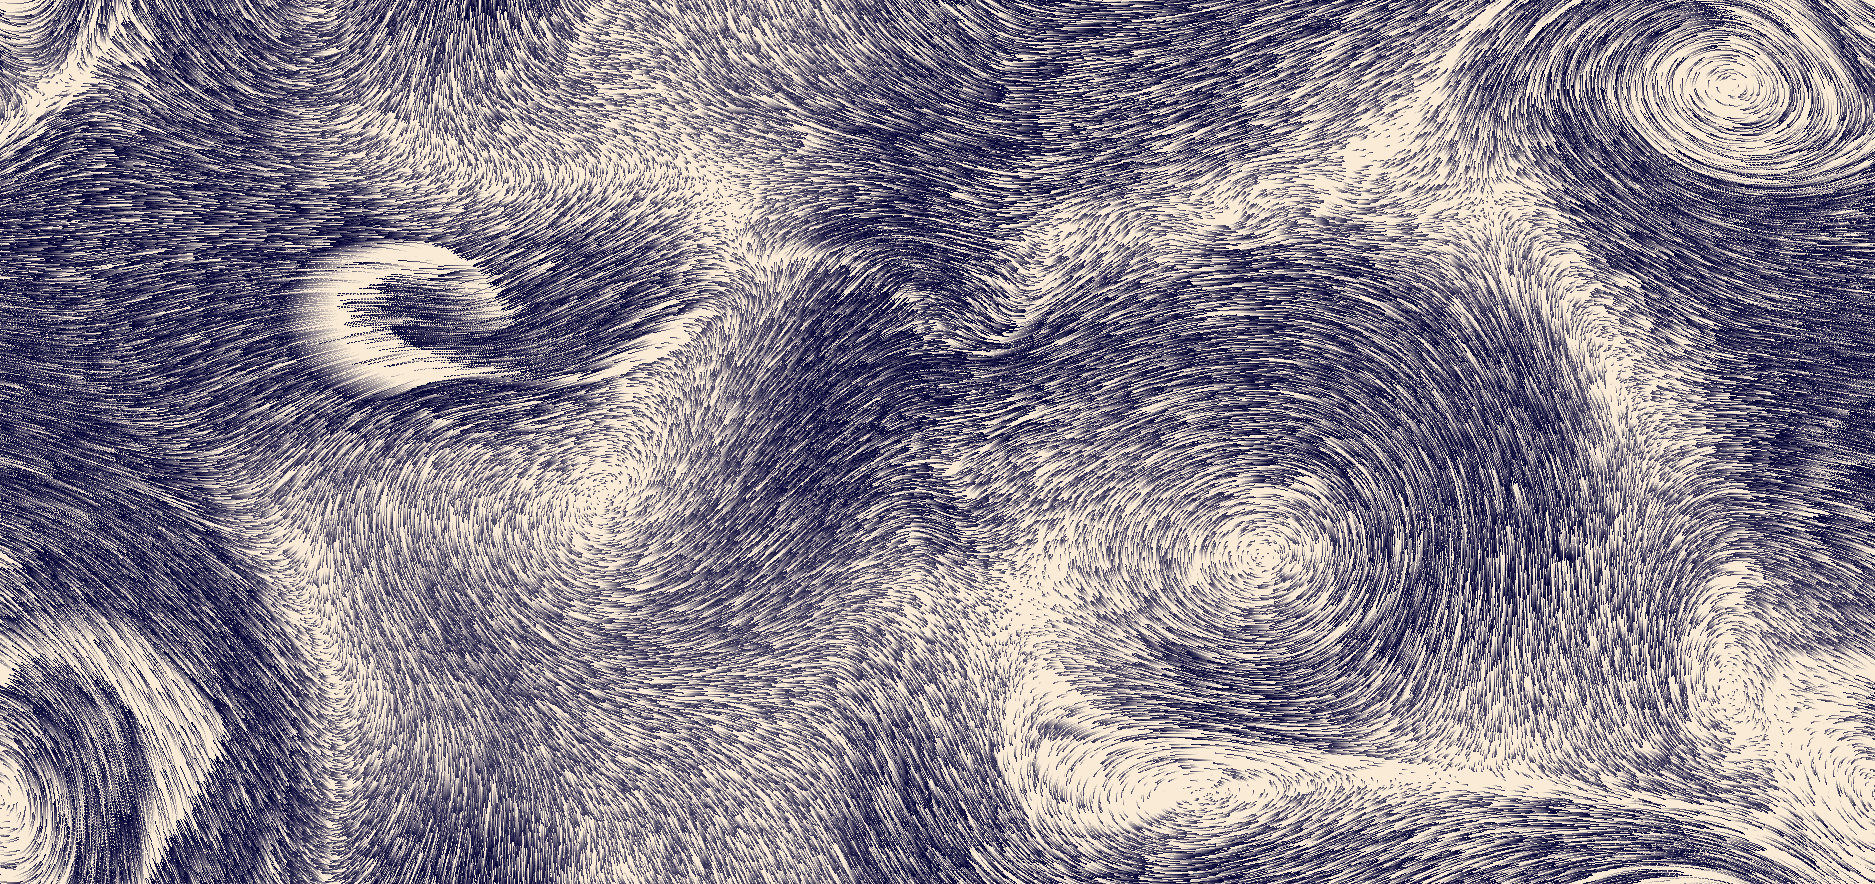
\includegraphics[width=0.4\linewidth]{Figuras/Desarrollo/MarParticulas.png}
	\caption{Referencia principal de arte interactivo en relación con la propuesta de Clara Guoshi, miembro de ARTEMIS. En el enlace de la referencia bibliográfica, se puede probar la experiencia creada por Vamoss.}
	\label{fig:SeaParticles}
\end{figure}

\section{Musicoterapia y composición interactiva}

La composición interactiva se basa en la creación de música como una forma de expresión libre. Mediante la modificación en tiempo real de un tema musical o combinaciones musicales, se pueden generar variaciones melódicas y paisajes sonoros. A través de esta interacción, el paciente puede crear música sencilla. Esta línea de investigación presenta dos aplicaciones. Aunque son diferentes, ambas buscan utilizar los mismos métodos para alcanzar el objetivo.

\subsection{Aplicación 1: Paisaje sonoro}

El paisaje sonoro, que se inspira en referencias como Reactable\footnote{Reactable es un instrumento musical electrónico colaborativo desarrollado por el Grupo de Tecnología Musical de la Universidad Pompeu Fabra en Barcelona. Este instrumento permite a los usuarios crear topologías musicales complejas y dinámicas mediante la colocación y rotación de elementos físicos en su interfaz. Está inspirado en los sintetizadores modulares de los años sesenta y permite el uso de generadores, filtros y moduladores para la creación musical.} o Incredibox (\citeauthor{INCREDIBOX:2023}, \citeyear{INCREDIBOX:2023}), se centra en la creación de música a través de la selección de los instrumentos que participarán en la melodía. Esta aplicación tiene como objetivo acomodar a aquellos pacientes con menor conocimiento musical, reforzando la simplicidad requerida para que estas aplicaciones sean utilizadas por su público objetivo. En realidad, no existe una solución incorrecta, lo que permite al paciente sentir que tiene el control de la música y evitar la frustración de no poder crear una melodía armoniosa.

La aplicación consta de cuatro niveles distintos, cada uno asociado a un género musical. Esto permite al terapeuta seleccionar los instrumentos con los que desea trabajar, en función de las necesidades del paciente. Además, la aplicación puede utilizarse de manera indefinida, hasta que el paciente o el terapeuta decidan finalizar su uso. La idea principal de la aplicación es que los instrumentos generan un paisaje musical, asociando cada elemento con aspectos de la naturaleza, como flores o árboles. Este paisaje cambia según el género musical seleccionado. Los cuatro géneros que agrupan los distintos instrumentos, junto con algunos ejemplos de instrumentos, son:

\begin{itemize}
	\item \textbf{Música clásica:} piano, violín, viola, trompeta, trombón, percusión, violonchelo, oboe, corno, fagot, clarinete, contrabajo, flauta traversa o flauta de pico.
	\item \textbf{Música pop-rock:} voz, guitarra eléctrica, bajo, batería, teclados, guitarra acústica, sintetizador o caja de ritmos.
	\item \textbf{Música caribeña o latina:} gaitas, arco musical, caña de millo, guacharaca, guache, tablitas, bombos, redoblantes, platillos, campanas o tambor.
	\item \textbf{Música electrónica:} sintetizador, caja de ritmos, theremin o sonidos generados por ordenador.
\end{itemize}

Cada uno de estos géneros representa un paisaje específico, aludiendo a las cuatro estaciones. Los elementos de fondo y la paleta de colores cambian, pero siempre se mantiene el aspecto natural.La aplicación, desarrollada por Ángela García, miembro de ARTEMIS, incluye un menú inicial donde se puede seleccionar el género deseado y la pantalla de juego, donde se puede observar en acción lo que hemos mencionado anteriormente. En la \autoref{fig:SonoricEnvironment}, se pueden observar ambas interfaces.

\begin{center}
	\textbf{Fuente:} Realizado por Ángela García, miembro ARTEMIS.
	\vspace{-18pt}
\end{center}

\begin{figure}[h!]
	\centering
	\subfigure{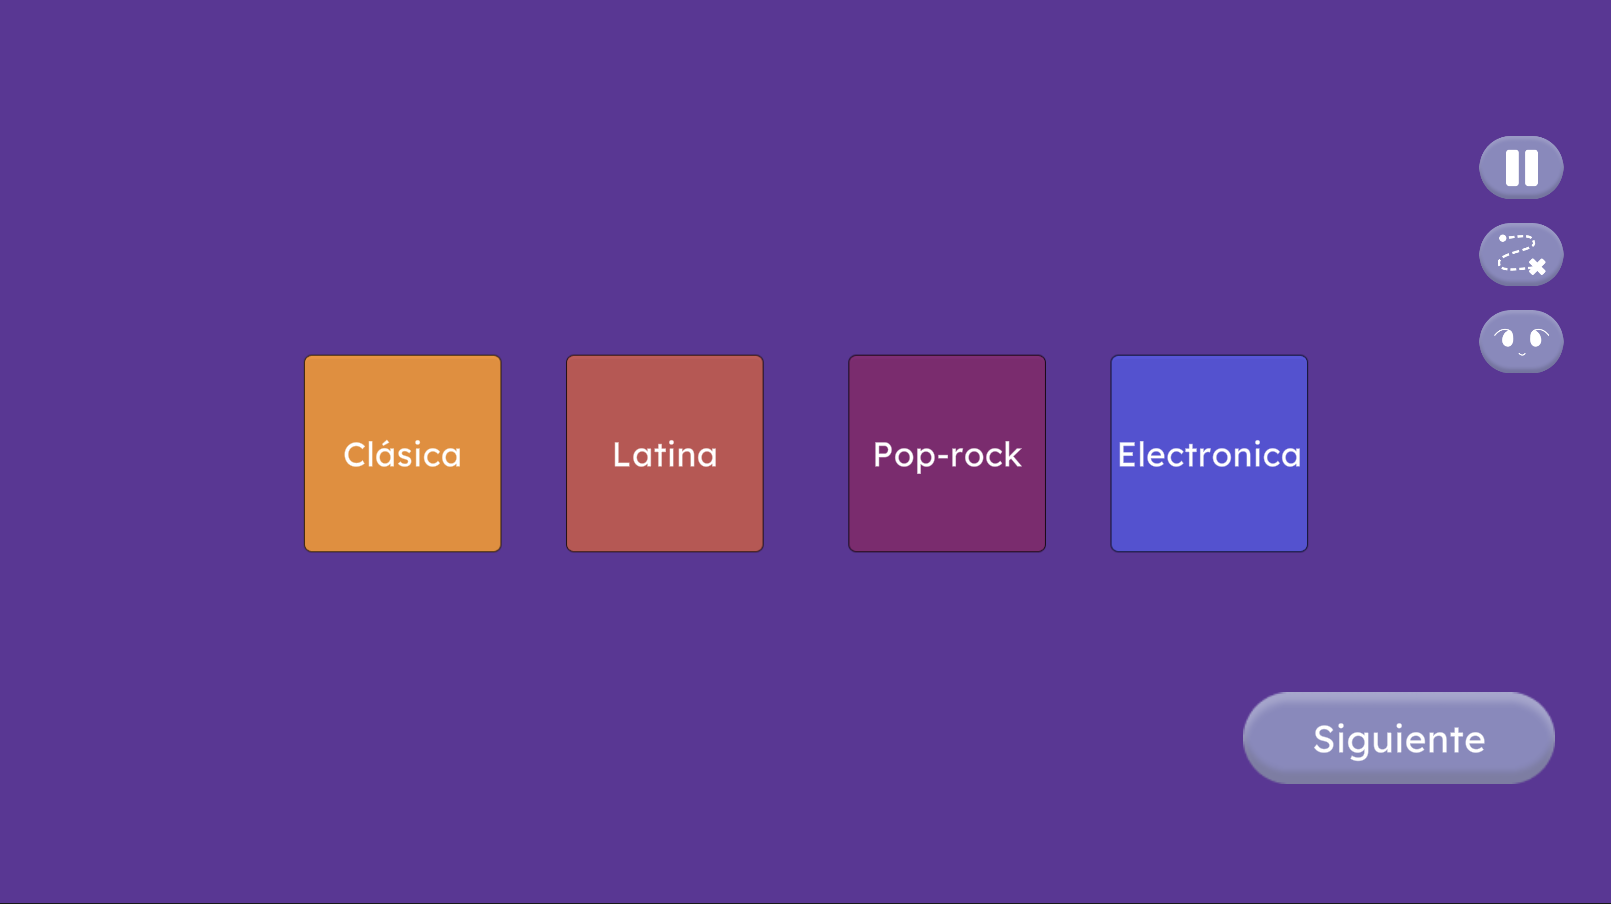
\includegraphics[width=0.4\textwidth]{./Figuras/Desarrollo/PaisajeSonoroMenu.png}\label{fig:SonoricEnvironmentMenu}}
	\hfil
	\subfigure{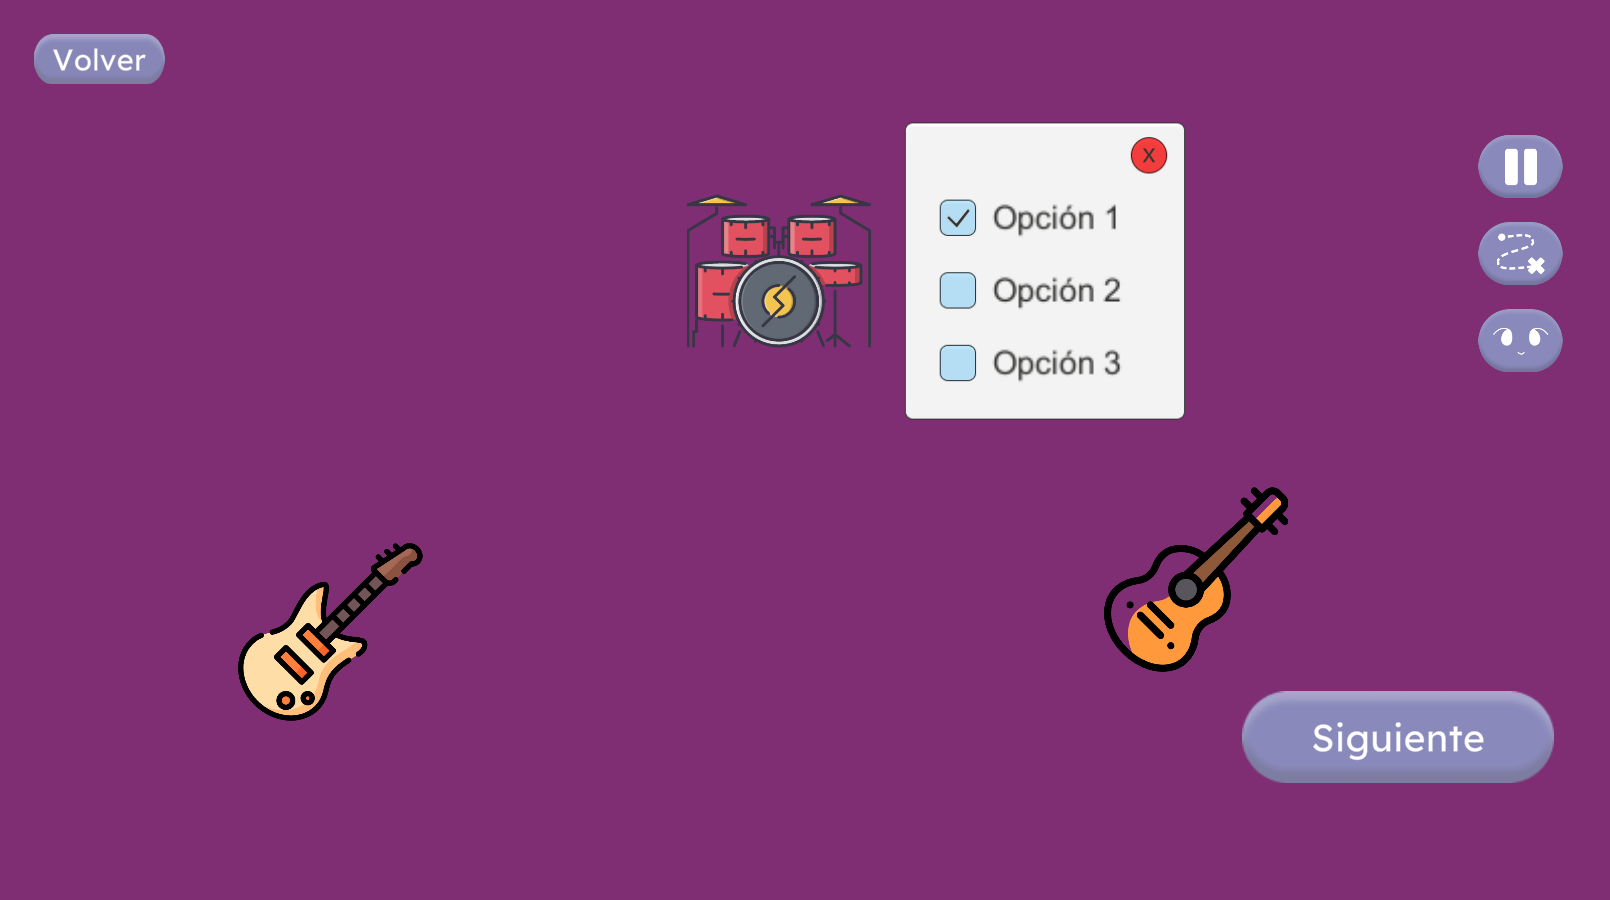
\includegraphics[width=0.4\textwidth]{./Figuras/Desarrollo/PaisajeSonoroGame.png}\label{fig:SonoricEnvironmentGame}}
	\caption{Pantallas del menú y del juego en la aplicación de paisaje sonoro.}
	\label{fig:SonoricEnvironment}
\end{figure}

\begin{center}
	\textbf{Fuente:} Realizado por Leticia Gómez, compositora ARTEMIS.
	\vspace{-14pt}
\end{center}

\begin{figure}[h!]
	\centering
	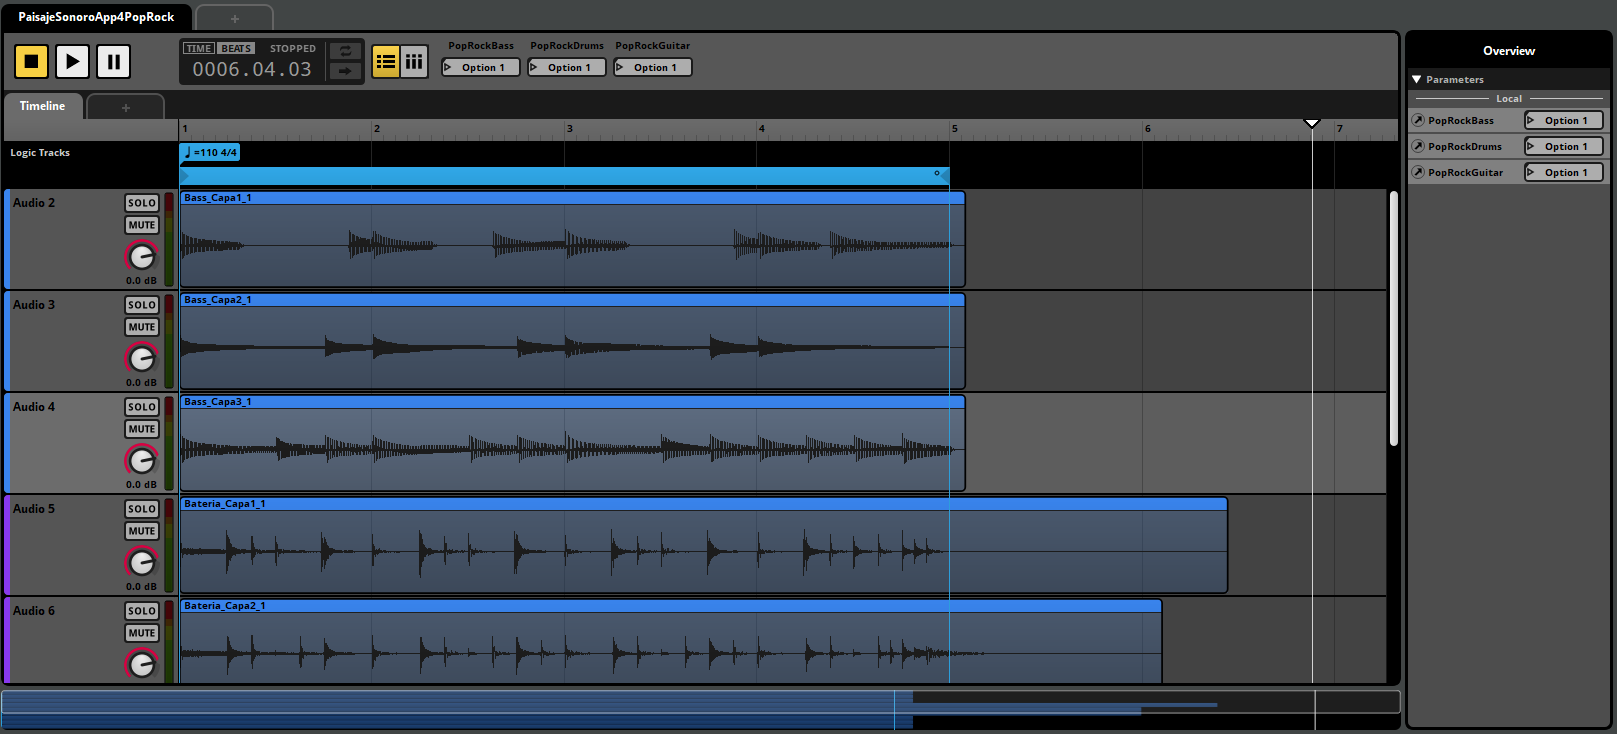
\includegraphics[width=0.8\linewidth]{Figuras/Desarrollo/PaisajeSonoroFMOD.png}
	\caption[Interfaz de FMOD aplicación paisaje sonoro.]{Interfaz de FMOD con los contenidos del género pop-rock de la aplicación de paisaje sonoro.}
	\label{fig:SonoricEnvironmentFMOD}
\end{figure}

A nivel musical, la aplicación utiliza FMOD para sincronizar rítmicamente las diversas pistas de audio y los parámetros para alternar entre ellas. Se puede observar en la \autoref{fig:SonoricEnvironmentFMOD}, cómo está configurado el middleware de audio para garantizar el correcto funcionamiento de la aplicación. Cada evento de FMOD engloba un género específico. Aquí se agrupan todas las pistas de audio por instrumentos, que se reproducen según los parámetros indicados a través de scripting dentro de Unity.

\subsection{Aplicación 2: Melodía floral}

A diferencia de la aplicación anterior, esta tiene una complejidad musical mayor, requiriendo un entendimiento teórico previo para su uso. Sin embargo, los conceptos utilizados en la aplicación son bastante sencillos para que un niño sin experiencia musical pueda aprenderlos rápidamente, tras una breve explicación del terapeuta. Al mismo tiempo, son lo suficientemente profundos para que un niño con experiencia musical pueda desenvolverse cómodamente con sus conocimientos adquiridos previamente. La aplicación de melodía floral incluye un pentagrama interactivo que permite cambiar tanto la duración como la altura de las notas. Por ello, es necesario conocer la nomenclatura musical, aunque no necesariamente de las notas, pero sí de los tipos de duración que existen, como las redondas, blancas, negras, corcheas, etc.

En cada iteración de la aplicación, se carga una melodía de una biblioteca, que el terapeuta puede seleccionar según las necesidades del paciente. Una vez seleccionada, aparece un pentagrama clásico con las notas dispuestas de acuerdo con la melodía. La estética de la aplicación conserva un aspecto natural, y cada nota se representa con un tipo de flor. La flor cambiará dependiendo de la duración de la nota, con las notas negras representadas por flores más oscuras y las notas blancas por flores literalmente blancas. Los silencios se representan con una hoja otoñal caída. Una gran referencia para la aplicación es el editor de melodías de Animal Crossing: New Horizons (\cite{ACNH:2020}), que permite la creación musical a través de la colocación de notas y silencios, variando la altura de las mismas.

\begin{center}
	\textbf{Fuente:} Realizado por Elisa Alonso, miembro ARTEMIS.
	\vspace{-18pt}
\end{center}

\begin{figure}[h!]
	\centering
	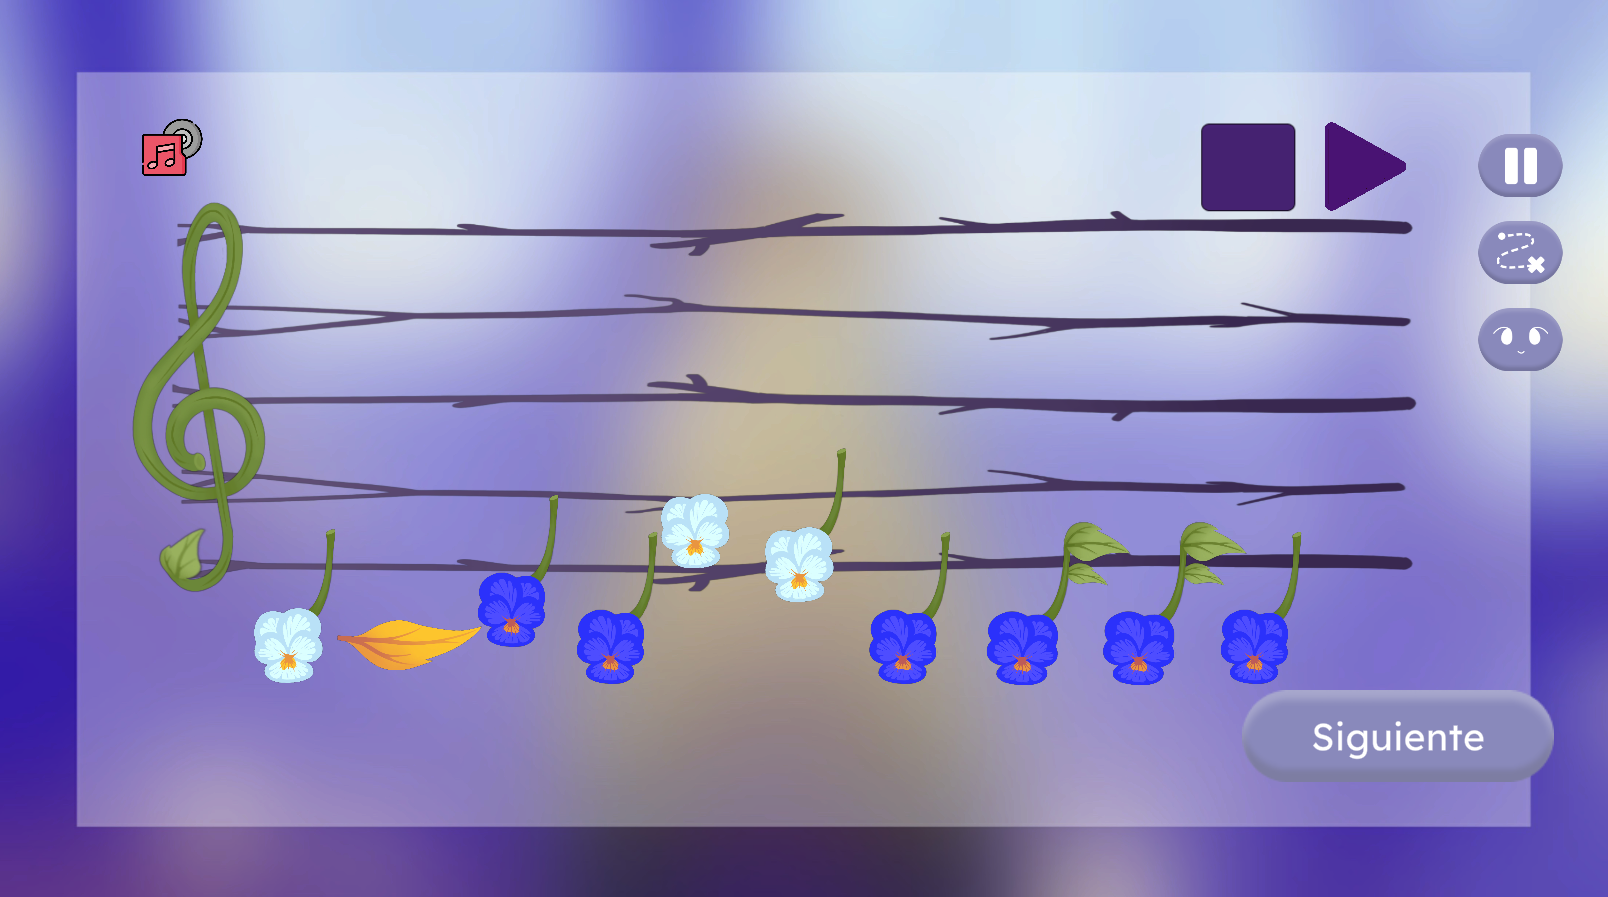
\includegraphics[width=0.6\linewidth]{Figuras/Desarrollo/MelodiaFloralGame.png}
	\caption[Interfaz de la aplicación melodía floral.]{Interfaz de la aplicación de melodía floral, mostrando un ejemplo de notas a distintas alturas y con diferentes figuras.}
	\label{fig:FloralMelodyGame}
\end{figure}



